	\documentclass[twoside]{article}
\usepackage{../../estilo-ejercicios}
\renewcommand{\baselinestretch}{1,3}
%--------------------------------------------------------
\begin{document}

\title{Problema para subir nota}
\author{Javier Aguilar Martín}
\maketitle

\begin{ejercicio}{1}
Sean $I = [0, 1]$, $M$ una banda de Möbius y $∂M ⊂ M$ su borde. Supongamos que
tenemos aplicaciones continuas inyectivas cualesquiera $f_1, f_2 : I → S^3$, $g : M → S^3$ y $h: \R P^2→ S^3$
tales que $\Ima f_1 ∩ \Ima f_2 = ∅$.
\begin{enumerate}[(a)]
\item Calcula $H_*(S^3 − \Ima f_1 ∪ \Ima f_2)$ obteniendo explícitamente generadores mediante ciclos representantes.
\item Halla $H_*(S^3 − \Ima g)$ estableciendo isomorfismos con grupos abelianos conocidos y determina el homomorfismo $H_*(S^3 − \Ima g) → H_*(S^3 − \Ima g|_{∂M} )$ inducido por la inclusión $∂M ⊂ M$.
\item Calcula $H_*(S^3−\R P^2)$. ¿Qué consecuencias puedes extraer de los resultados obtenidos?
\end{enumerate}
\end{ejercicio}
\begin{solucion}
Las aplicaciones  inyectivas entre espacios compactos y Hausdorff son homeomorfismos sobre sus imágenes, lo cual ocurre en todas las aplicaciones del enunciado. 
%En el ejercicio vamos a usar levemente el teorema 3.44 de Hatcher:
%
%\begin{teorema}
%Si $K$ es un subespacio compacto y localmente contrácil de una $n$-variedad cerrrada, entonces $H_i(M,M-K;\Z)\cong H^{n-i}(K;\Z)$ para todo $i$.
%\end{teorema}
%
%De este teorema se deduce que si $A$ y $B$ son dos subespacios de $M$ compactos y localmente contráctiles homeomorfos entre sí, entonces $H_i(M,M-A;\Z)\cong H^{n-i}(A;\Z)\cong H^{n-i}(B;\Z)\cong H_i(M,M-B;\Z)$. 
%
%En nuestro caso, todos los espacios que se consideran son compactos y localmente contráctiles (son de hecho localmente euclídeos) y $S^3$ es una 3-variedad cerrada y orientable. Además, las aplicaciones  inyectivas entre espacios compactos y Hausdorff son homeomorfismos sobre sus imágenes (son embebimientos). Así que por lo que hemos deducido del teorema, podemos sustituir $f_1$, $f_2$, $g$ y $h$ por cualesquiera otros embebimientos siempre que se verifique que las imágenes de los sustitutos de $f_1$ y $f_2$ sean disjuntas. 
%
%En realidad se podría resolver la mayor parte del problema aplicando directamente el teorema, pero vamos a tratar de hacerlo de forma más elemental para extraer información sobre los generadores y los homomorfismos inducidos. 

%VOY A USAR DUALIDAD DE ALEXANDER \url{https://math.stackexchange.com/questions/3121316/if-a-and-b-are-homeomorphic-proper-closed-subsets-of-mathbbrn-do-thei}
%\url{https://math.stackexchange.com/questions/877003/homology-of-3-sphere-minus-an-embedding-of-s1-times-mathbbd2}
%https://math.stackexchange.com/questions/195848/homeomorphism-question-relating-to-the-topological-3-sphere

%PARA CUBRIR COSAS CON BOLAS PUEDE QUE NECESITE ARGUMENTAR ESTO \url{https://en.wikipedia.org/wiki/Normal_space}
%LOS ESPACIOS SON LOCALMENTE CONTRACTILES \url{https://topospaces.subwiki.org/wiki/Locally_contractible_space} Y POR TANTO PUEDO USAR DUALIDAD DE ALEXANDER (3.44 HATCHER) EL COROLARIO 3.45 ES LA POLLAAAAAAA
\begin{enumerate}[(a)]
%\item Por ser $f_1$ y $f_2$ aplicaciones inyectivas entre espacios compactos y Hausdorff, tenemos que son homeomorfismos sobre sus imágenes, pues $f_i:I\to f_i(I)$ es biyectiva, continua y cerrada. AUNQUE SEAN HOMEOMORFOS, EL COMPLEMENTARIO NO TIENE POR QUÉ SERLO, COMO PASA CON LA ESFERA DE ALEXANDER, MIRAR EL TEORMA DE LA CURVA DE JORDAN GENERALIZADO (2B.1) INTENTAR COMBINARLO CON MAYER-VIERTORIS. PUEDE SERVIRME ADAPTAR THEOREM 7.8 DE MADSEN A LA ESFERA, AL MENOS PARA EL 0
\item Como $\Ima f_1\cap\Ima f_2=\emptyset$, ambos homeomorfos a $I$ y $S^3$ es metrizable, podemos considerar entornos tubulares disjuntos $N_1$ de $\Ima f_1$ y $N_2$ de $\Ima f_2$ en $S^3$. Estos entornos son contráctiles. Sea entonces $A=N_1\cup N_2$ y $B=S^3-\Ima f_1\cup \Ima f_2$. Tenemos que $A\cup B=S^3$ y $A\cap B\simeq S^2\sqcup S^2$. Tenemos que $H_0(B)=\Z$ ya que el espacio es claramente conexo por caminos, así que esta homología está generada por cualquier símplice singular $\sigma:\Delta^0\to B$. Por la sucesión de Mayer-Vietoris, el único otro grupo de homología no trivial se encuentra en la sucesión exacta
\[
0\to H_3(S^3)\to H_2(S^2\sqcup S^2)\to 0\oplus H_2(B)\to 0
\]
que podemos reescribirla como
\[
0\to\Z\to \Z\oplus\Z\to H_2(B)\to 0
\]
Vamos a deducir que $H_2(B)=\Z$, para lo cual comprobaremos que la aplicación $\partial: H_3(S^3)\to H_2(S^2\sqcup S^2)$ es en realidad la aplicación $1\mapsto (1,1)$. Atendiendo a las observaciones de la página 150 de Hatcher, podemos subdividir $\Delta^3$ de modo que el generador $\alpha$ de $H_3(S^3)$ inducido por $q:\Delta^3\to S^3$ se pueda representar por un ciclo de la forma $x+y$, donde $x\in C_3(A)$ e $y\in C_3(B)$, de modo que $\partial\alpha =[d(x)]\in H_2(A\cap B)$. En concreto, podemos tomar una subdivisión de modo que $d(x)$ sea la suma de los generadores de cada una de las copias de $S^2$ en $A\cap B$, considerando un subcomplejo de la subdivisión de $\Delta^3$ en su interior cuya imagen esté enteramente contenida en $A$ y cuyo borde sea homeomorfo a las esferas contenidas en $A\cap B$. De esta forma, conseguimos que efectivamente $\partial(1)=(1,1)$. 

\begin{figure}[h!]
\centering
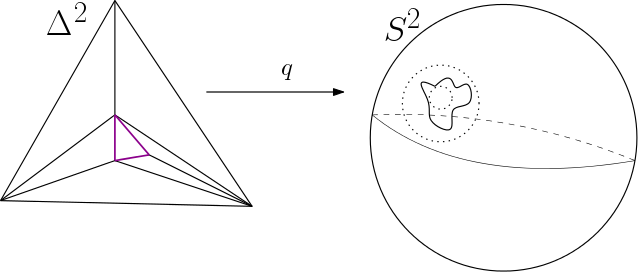
\includegraphics[scale=0.6]{dibujo}
\caption{Dibujo sustituyendo $S^3$ por $S^2$ y una de las copias de $S^2$ por una copia de $S^1$. El triángulo morado se envía mediante la aplicación cociente al interior del entorno punteando de mayor tamaño, de modo que al eliminar el entorno punteado pequeño se convierte en un generador.}
\end{figure}

Así, considerando en $\Z\oplus\Z$ la base $\{(1,0), (1,1)\}$, tenemos que $H_2(B)\cong \Z$. Podemos entonces tomar como generador de $H_2(B)$ la imagen mediante $\varphi: H_2(S^2\sqcup S^2)\to H_2(B)$ de cualquiera de los dos generadores usuales de $H_2(S^2\sqcup S^2)$, ya que en $H_2(B)$ representan el mismo elemento. Además, por cómo está definido el homomorfismo $\varphi$, el ciclo generador en $H_2(B)$ es exactamente el mismo que en $H_2(S^2\sqcup S^2)$ (o con signo opuesto). 

%TENGO QUE VER CON LO DE LA PÁGINA 150 CÓMO ACTÚA EL HOMOMORFISMO DE CONEXION, SUBDIVIDIENDO PARA QUE ALGO ENTRE EN A Y VER QUE EFECTIVAMENTE ENTRA DE MODO QUE EL COCIENTE ES LIBRE DE TORSION

 %QUE REPRESENTEN EL MISMO O QUE UNO SE VAYA O QUE SEA UNO UN MÚLTIPLO DE OTRO DEPENDERÁ EN REALIDAD DE LO DE ANTES


\item Consideramos ahora un entorno tubular $N$ de $\Ima g$, que será homeomorfo al interior de un toro sólido, posiblemente anudado, pero en cualquier caso homotópico a $S^1$. Sean entonces $A=N$ y $B=S^3-\Ima g$. Tenemos entonces que $A\cup B=S^3$ y $A\cap B\simeq T^2$ (un toro). Claramente $B$ es conexo por caminos, por lo que $H_0(B)=\Z$. Calculamos el resto de grupos usando Mayer-Vietoris, de donde se deduce fácilmente que $H_i(B)=0$ para $i\geq 3$. Empezamos calculando $H_1(B)$ a partir de la sucesión exacta
\[
0\to H_1(A\cap B)\to H_1(A)\oplus H_1(B)\to 0,
\]
de donde $\Z\oplus\Z = H_1(A\cap B)\cong H_1(A)\oplus H_1(B)=\Z\oplus H_1(B)$, por lo que necesariamente $H_1(B)\cong\Z$. Por último, para $H_2(B)$ tenemos la sucesión exacta
\[
0\to H_3(S^3)\to H_2(A\cap B)\to H_2(A)\oplus H_2(B)\to 0
\]
que se reescribe como
\[
0\to \Z\to \Z\to H_2(B)\to 0
\]
Con un procedimiento similar al del apartado anterior, podemos probar ahora que la aplicación $\Z\to\Z$ es sobreyectiva y por tanto $H_2(B)=0$. Para ello, basta subdividir $\Delta^3$ y considerar un subcomplejo homeomorfo a un toro sólido en el interior de $\Delta^3$ que se envíe a $N$ mediante la aplicación cociente $\Delta^3\to S^3$. De este modo, si escribimos $\alpha=[x+y]$ como en el apartado anterior, donde $x$ es la cadena que se ha descrito, entonces $[d(x)]$ es el generador de $H_2(A\cap B)$. \\


Buscamos ahora el homomorfismo $H_*(S^3 − \Ima g) → H_*(S^3 − \Ima g|_{∂M} )$ inducido por la inclusión $∂M ⊂ M$. Obsérvese que $H_*(S^3 − \Ima g|_{∂M} )$  se calcula exactamente igual que hemos calculado $H_*(S^3 − \Ima g)$, ya que podemos tomar el mismo entorno tubular $N$ y el resto de cálculos no se ven afectados. Como el homomorfismo $H_0(S^3 − \Ima g) → H_0(S^3 − \Ima g|_{∂M} )$ es claramente la identidad, solo tenemos que determinar $$H_1(S^3 − \Ima g) → H_1(S^3 − \Ima g|_{∂M} ),$$ pues los demás son triviales. Usando los cálculos anteriores y lo que hemos mencionado sobre que para $S^3 − \Ima g|_{∂M}$ serían los mismos cálculos, tenemos el cuadrado conmutativo
\[
\begin{tikzcd}
H_1(A\cap (S^3-\Ima g))\arrow[r, "\cong"]\arrow[d, "\cong"] & H_1(A)\oplus H_1(S^3-g(M))\arrow[d, "1\oplus i_*"]\\
H_1(A\cap (S^3 − \Ima g|_{∂M} ))\arrow[r, "\cong"] & H_1(A)\oplus H_1(S^3 − \Ima g|_{∂M} )
\end{tikzcd}
\]
Los isomorfismos horizontales se obtuvieron en el cálculo de la homología y el isomorfismo vertical izquierdo está inducido por la inclusión al ser ambos espacios homotópicamente equivalentes al toro $T^2$. Por conmutatividad, $i_*$ es un isomorfismo $\Z\to\Z$ y por tanto es la identidad si elegimos generadores adecuados (podría ser el opuesto a la identidad). 

%\url{https://math.stackexchange.com/questions/1620689/complement-of-the-solid-torus-in-s3-is-again-a-solid-torus}
%\item Por el mismo argumento del principio del anterior ejercicio, $g$ es homeomorfismo sobre su imagen. 
%
%\url{https://math.stackexchange.com/questions/3017199/homology-and-mobius-band}
\newpage

\item Sabemos que $\R P^2 = M\cup D^2$, por lo que $S^3-M=(S^3-\R P^2)\cup D^2$, verificándose además $(S^3-\R P^2)\cap D^2=\emptyset$. Utilizamos el cálculo de la homología de $S^3-M$ para calcular la de $S^3-\R P^2$ por Mayer-Vietoris. Obtenemos inmediatamente que $H_i(S^3-\R P^2)=0$ para $i\geq 2$. Para $i=1$ la calculamos usando la sucesión exacta
\[
0\to H_1(S^3-\R P^2)\oplus H_1(D^2)\to H_1(S^3-M)\to 0
\]
o lo que es lo mismo
\[
0\to H_1(S^3-\R P^2)\to \Z\to 0
\]
por lo que $H_1(S^3-\R P^2)\cong \Z$. Por último, para $i=0$ tenemos
\[
0\to H_0(S^3-\R P^2)\oplus H_0(D^2)\to H_0(S^3-M)\to 0
\]
que es equivalente a 
\[
0\to H_0(S^3-\R P^2)\oplus \Z\to \Z\to 0
\]
de donde deducimos que $H_0(S^3-\R P^2)=0$. De aquí obtenemos al menos dos contradicciones con lo que tenemos hasta el momento. En primer lugar, este último resultado implica que $S^3-\R P^2=\emptyset$, pero $H_1(\emptyset)=0$, lo que entra en contradicción con que $H_1(S^3-\R P^2)=\Z$. También tenemos otra contradicción para la cual no necesitamos ninguna otra homología. Como estamos identificando $\R P^2$ con un embebimiento suyo en $S^3$, el hecho de que $S^3-\R P^2=\emptyset$ significaría que $S^3\cong \R P^2$, lo cual sabemos que es falso. La conclusión es por tanto que no puede existir $h:\R P^2\to S^3$ inyectiva, es decir, $\R P^2$ no puede embeberse en $S^3$. 
%De nuevo $h$ es homeomorfismo sobre su imagen. 
%
%CREO QUE DEBO LLEGAR A LA CONCLUSIÓN DE QUE $h$ NO PUEDE EXISTIR, PORQUE SEGÚN EL COROLARIO 3.46 NO SE PUEDE EMBEBER EN $\mathbb{R}^3$ Y POR TANTO TAMPOCO EN $S^3$, YA QUE SI SE PUDIERA, NO SERÍA SOBREYECTIVO PORQUE NO SON HOMEOMORFOS Y ENTONCES LA PROYECCIÓN ESTEREOGRÁFICA DARÍA UN EMBEBIMIENTO EN $\R^3$. POR EJEMPLO, SI USARA EL 3.45 SALDRÍA DIRECTAMENTE UNA CONTRADICCIÓN PORQUE $H^2=\Z_2$ Y LA REDUCIDA EN 0 ES 0 PORQUE QUITARLE UN CONEXO ACOTADO POR UNA BOLA PROPIA QUEDA CONEXO, PERO SUPONGO QUE NO PUEDO UTILIZAR ESTO. 
\end{enumerate}

\begin{nota}
Usando la dualidad de Alexander (teorema 3.44 de Hatcher) los cálculos son inmediatos, así como la conclusión de $\R P^2$ no puede ser embebido en $S^3$, pero obtenemos menos información geométrica y además no hemos visto ese resultado en clase.
\end{nota}

%\url{https://math.stackexchange.com/questions/1354119/are-the-complements-of-two-homeomorphic-compact-connected-subsets-of-mathbbr}
%\url{https://math.stackexchange.com/questions/43096/is-it-true-that-a-space-filling-curve-cannot-be-injective-everywhere}
%\url{https://proofwiki.org/wiki/Baire_Category_Theorem}
\end{solucion}

\end{document}
